\documentclass{jsarticle}

\usepackage{listings,jlisting}
\usepackage[dvipdfmx]{graphicx}
\usepackage{bmpsize}
\usepackage{bm}
\usepackage{here}

\lstset{
    basicstyle={\ttfamily},
    identifierstyle={\small},
    commentstyle={\smallitshape},
    keywordstyle={\small\bfseries},
    ndkeywordstyle={\small},
    stringstyle={\small\ttfamily},
    frame={tb},
    breaklines=true,
    columns=[l]{fullflexible},
    numbers=left,
    xrightmargin=0zw,
    xleftmargin=3zw,
    numberstyle={\scriptsize},
    stepnumber=1,
    numbersep=1zw,
    lineskip=-0.5ex
}
\begin{document}

\title{計算機科学実験及演習4 エージェント 課題4}
\author{1029-28-2473 二見 颯}
\maketitle

% 相互情報量を用いた特徴選択
% Bayes 最適化によるハイパーパラメータ選択

\section{課題4-1}
\subsection{プログラム概要}
リスティングデータによって与えられる類似の宿泊施設の提示価格を予測して、それによって自己の宿泊施設の価格推薦を
行うことを考える。
民泊市場にはリスティングデータに従う貸し手1人と価格推薦エージェント1体という条件で、価格推薦エージェントはリスティングデータの
価格を予測して、それより少し価格を提示するとする。

\subsection{外部仕様}
リスティングデータとして、San Francisco-listings.csv を用いることとする。 \\
課題3と同様に、96の特徴量のうち
'latitude', 'longitude', 'accommodates', 'property\_type', 'room\_type', 'number\_of\_reviews', 'review\_scores\_rating'を説明変数
として、'price' を目的変数とする。ただし、'price' が 500 以下のデータのみを利用する。 \\
bayes\_opt.py\\
{\bf pip install scikit-optimize} が必要。 \\
Grid Search の代わりにベイズ最適化の手法を用いて、SVR の最適なハイパーパラメータを探索する。\\
agent.py \\
予測価格の何\%とするかをコマンドライン引数として取り、SVR による価格予測を用いて価格推薦を行う1体のエージェントを
シミュレーションする。
プログラムの実行は \\
{\bf ./agent.py [percentage]} \\
とする。
以下は agent.py の実行例である。
\begin{lstlisting}
$ ./agent.py 90
load sanfrancisco: read 1000 / 6196 data
start SVR fit...
cvxopt.solvers.qp: optimization succeeded
start SVR predict...
revenue by SVR agent:  24257.254376011988
the agent wins 298 times
mean of y_train:  172.424
revenue of mean price offering:  17343.63600000005
the agent wins 189 times
\end{lstlisting}

\subsection{内部仕様}
\subsubsection*{bayes\_opt.py}
load\_sanfrancisco関数によってSan Francisco-listing.csv を読み込み、データの前処理ののちに
X\_pro, y\_proを得る。

spaces には SVR の各パラメータ(p, C, eps)の定義域を与えて、skopt.gp\_minimizeにより
bayes\_opt関数を最小化するようなパラメータを探索する。

bayes\_opt では与えられたパラメータのSVRを構成して、交差検証によって得た決定係数(5回の平均)
に-1を掛けたものを返す。(決定係数は1に近づくように最大化したいため)

\subsubsection*{agent.py}
load\_sanfrancisco関数によって得たX, yについて、前半を訓練データ、後半を評価データとする。

bayes\_opt.pyによって発見した最適なパラメータでSVRを構成して、訓練データによってSVRを学習させ、
それによって評価データを予測する。

コマンドライン引数を$m$として、SVRによる予測価格の$m$\%が提示価格となる。

リストの価格の30\%は原価として考えて、各提示価格について提示価格がリストの価格を下回ったときに
(提示価格 - リストの価格 * 0.3)が利益となる。これらの総利益をエージェントの評価基準とする。
利益はマイナス(すなわち赤字)となることも考えられる。

\subsection{評価結果}
% 各説明変数と price の相関
選択した説明変数のうち数値データ('latitude', 'longitude', 'accommodates', 'number\_of\_reviews',
'review\_scores\_rating')と目的変数'price'との相関を図1に示す。
\begin{figure}[H]
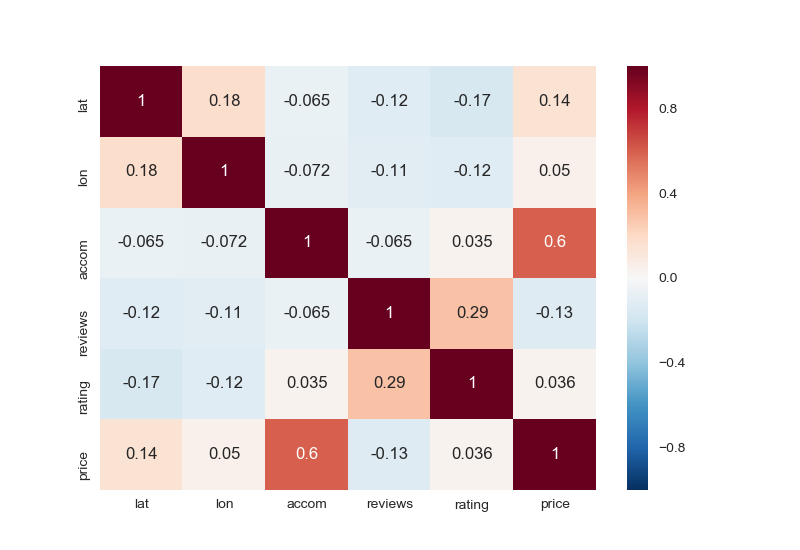
\includegraphics[width=15cm]{corr.png}
\caption{Correlation coefficient}
\end{figure}

% ベイズ最適化
SVR の予測精度(決定係数)についてベイズ最適化により最適なハイパーパラメータ$C, \sigma, \epsilon$を探索した。
探索範囲は$2^{-1} \leq \sigma \leq 2^5$, $2^{-5} \leq C \leq 2^{15}$, $2^{-10} \leq \epsilon \leq 2^{-3}$である。
図2にベイズ最適化で探索したパラメータ$C, \sigma$とそのときの決定係数の値を示す。(データ数は500で100回探索した)
\begin{figure}[H]
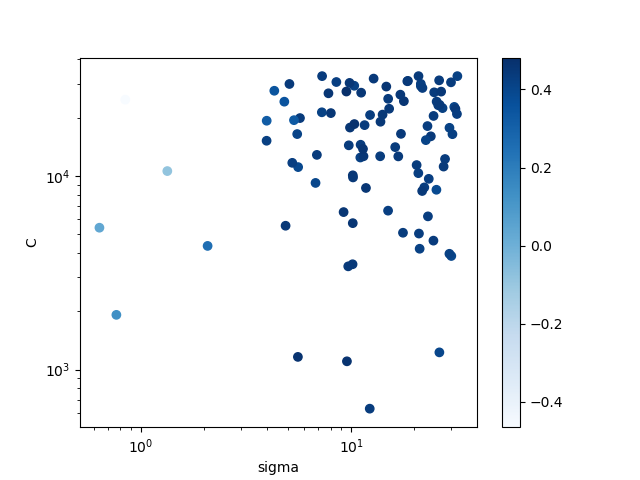
\includegraphics[width=15cm]{bayes_opt.png}
\caption{Bayes Optimization}
\end{figure}
決定係数は$\sigma = 9.50, C = 2.73 * 10^4, \epsilon = 9.27 * 10^{-2}$のときに0.481と最大になった。

データ数2000をSanFrainciscoリスティングデータからサンプリングして、その前半1000個を訓練データ、後半1000個を
評価データとした。提示価格を予測価格の何\%とするかを変化させた時の総利益の変化を表1に示す。
\begin{table}[H]
    \centering
    \begin{tabular}{|r||c|c|c|} \hline
      (\%) & 総利益 & 成功回数 & 効率(総利益/成功回数) \\ \hline
      70 & 44470 & 837 & 53.1 \\
      75 & 47421 & 793 & 59.7 \\
      80 & 48558 & 739 & 65.7 \\
      85 & 49322 & 689 & 71.5 \\
      90 & 48622 & 629 & 77.3 \\
      95 & 47511 & 568 & 83.6 \\
      100 & 46029 & 510 & 90.2 \\
      105 & 42665 & 449 & 95.0 \\
      110 & 39205 & 394 & 99.5 \\
      115 & 37179 & 351 & 105.9 \\
      120 & 35160 & 313 & 112.3 \\ \hline
      mean & 33871 & 359 & 94.3 \\ \hline
    \end{tabular}
    \caption{agent by percentage}
\end{table}

\section{課題4-2}
\subsection{プログラム概要}
リスティングデータに従う貸し手1人と価格推薦エージェント1, エージェント2が存在するとする。
エージェントが最安の値段をつけたときに借り手がついて、収入が得られるとする。
ベイズ最適化で最も精度が良かったパラメータのSVRを利用したものをエージェント1、あまり精度が良くない
SVRを利用したものをエージェント2とする。

\subsection{外部仕様}
{\bf ./multiagent.py} で実行する。
以下は multiagent.py の実行例である。
エージェント1, 2の予測精度(決定係数), 総利益, 成功回数, 効率(総利益/成功回数)を
出力する。
\begin{lstlisting}
$ ./multi_agent.py 
load sanfrancisco: read 2000 / 6196 data
=== SVRAgent start ===
1 th cross validation...
cvxopt.solvers.qp: optimization succeeded
R2 score:  0.4797468020396928
2 th cross validation...
cvxopt.solvers.qp: optimization succeeded
R2 score:  0.33178028654882397
3 th cross validation...
cvxopt.solvers.qp: optimization succeeded
R2 score:  0.4714137117838899
4 th cross validation...
cvxopt.solvers.qp: optimization succeeded
R2 score:  0.49906353860044683
5 th cross validation...
cvxopt.solvers.qp: optimization succeeded
R2 score:  0.31606765685527194
5-fold average score:  0.41961439916562504
cross val score:  0.41961439916562504
start SVR fit...
cvxopt.solvers.qp: optimization succeeded
start SVR predict...
=== SVRAgent start ===
1 th cross validation...
cvxopt.solvers.qp: optimization succeeded
R2 score:  -0.05695700854191843
2 th cross validation...
cvxopt.solvers.qp: optimization succeeded
R2 score:  0.03379843202281596
3 th cross validation...
cvxopt.solvers.qp: optimization succeeded
R2 score:  -0.00822695472188295
4 th cross validation...
cvxopt.solvers.qp: optimization succeeded
R2 score:  0.06128181455545334
5 th cross validation...
cvxopt.solvers.qp: optimization succeeded
R2 score:  0.017475693763498
5-fold average score:  0.009474395415593185
cross val score:  0.009474395415593185
start SVR fit...
cvxopt.solvers.qp: optimization succeeded
start SVR predict...
revenue by SVR agent1:  16242.43831357982
the agent1 wins 340/1000 times
revenue1 per 1:  47.77187739288182
revenue by SVR agent2:  23875.955321474925
the agent2 wins 436/1000 times
revenue2 per 1:  54.761365416226894
\end{lstlisting}

\subsection{内部仕様}
\subsubsection*{multi\_agent.py}
load\_sanfrancisco関数によってSan Francisco-listing.csv を読み込み、データの前処理ののちに
X, yを得る。

load\_sanfrancisco関数によって得たX, yについて、前半を訓練データ、後半を評価データとする。

SVRAgent関数はパラメータを引数にとって、交差検証で精度を示したのち
訓練データで学習、評価データの予測を行う。提示価格は予測価格の85\%とする。

エージェント1, エージェント2, リスティングデータの価格のうち、最小のものに借り手がつくとする。
エージェントに借り手がついた場合、(提示価格 - リストの価格 * 0.3)がエージェントの利益となる。
\subsection{評価結果}
% 精度の良いエージェント1 vs 精度の悪いエージェント2
精度の良いAgent1($\sigma = 9.50, C = 2.70 * 10^4, \epsilon = 9.00 * 10^{-2}$)と
精度のあまり良くないAgent2($\sigma = 1.0, C = 1.0, \epsilon = 0.1$)
の総利益, 成功回数, 効率は表2のようになった。サンプリングされたデータを変更して5回実行した。
\begin{table}[H]
    \centering
    \begin{tabular}{|c||c|c||c||c|c|} \hline
      (Agent1)決定係数 & 総利益 & 成功回数 & (Agent2)決定係数 & 総利益 & 成功回数 \\ \hline
      0.419 & 16242 & 340 & 0.00947 & 23875 & 436 \\
      0.473 & 19088 & 386 & 0.0000350 & 23035 & 396 \\
      0.528 & 17584 & 384 & 0.0115 & 24607 & 422 \\
      0.486 & 17119 & 338 & 0.0175 & 24666 & 439 \\
      0.442 & 16432 & 330 & -0.0013 & 24807 & 450 \\ \hline
    \end{tabular}
    \caption{Agent1 vs Agent2}
\end{table}

\section{考察(課題4-1 + 課題4-2)}
課題4-1では、表1より提示価格を予測価格の85\%とした場合が総利益が最大になった。
提示価格の予測価格に対する割合を下げることで、予測価格がリスティングデータの価格より高い場合にも提示価格が予測価格を下回る場合が多くなり、
成功回数は上がるが、一回の提供あたりの利益が小さくなる。そのトレードオフを考慮して85\%あたりが望ましい。

課題4-2で2つのエージェントが存在する場合、どちらのエージェントが他より利益を上げることができるかは単純に決定することはできない。
(予測精度が高い方が総利益が常に高くなるとはいえない)
価格の予測精度が低くても他のエージェントとリスティングデータの価格より低い価格を提示することができれば、
利益を得ることができて、他のエージェントはそのとき利益を逃すからである。原価(30\%)を下回らない範囲で最低の価格を提示するような
エージェントがあれば、他のエージェントはどんなに正確に価格予測してリスティングデータに対し大きな利益が得られるような提示を行っても、
それを得る機会を失い、最終的に原価に近い価格を提示し続けたエージェントが最大の総利益を得る。

しかし、このように価格競争が発生して提示価格は限りなく原価に近づいた場合、
一方のエージェントが価格競争に勝利して全ての借り手に民泊を提供できたとしても
ほとんど利益を上げられなくなる。
それぞれのエージェントが自身の利益を追求すると、エージェント全体の利益は最小化されてしまう。(囚人のジレンマといえる)

一方、お互いのエージェントが交代で市場に参加すれば、それぞれのエージェントは借り手を
独占することはできないが、結果的に総利益を最大にできることがある。

\subsection{ベイズ最適化}
ハイパーパラメータの探索において、一般的な手法としてグリッドサーチがある。
グリッドサーチは離散的なパラメータの組の候補について全探索を行う。
一方、ベイズ最適化では、ある連続的な定義域をもつ入力(パラメータ)$x$に対して、
ブラックボックス関数$y = f(x)$を最小化(あるいは最大化)するような$x$を逐次的に求める手法である。
次の観測点$x$の候補の求め方は全探索ではなく、これまでの関数の評価値に基づいて判断する。

次の観測点を決定する戦略として、ここではEI戦略を用いた。
EI(期待改善量)戦略では、評価値$y$とこれまでで最高の評価値$y_{best}$として、
$y - y_{best}$の期待値(獲得関数)が最も高くなる点を次に観測する。
ブラックボックス関数はガウス過程に従うと仮定して、これまでの観測点から
信頼区間を形成して、関数の形をある程度予想することを考える。(図3, 参考文献5より)
\begin{figure}[H]
\centering
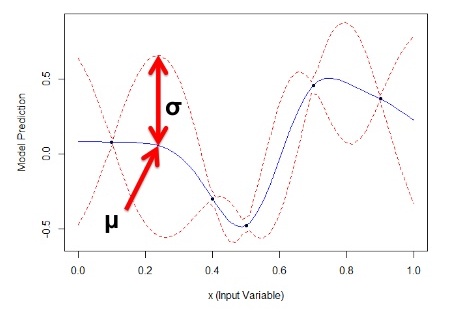
\includegraphics[width=10cm]{gauss.jpg}
\caption{Gaussian process}
\end{figure}
未観測点の期待値$\mu$と分散$\sigma^2$を計算すると、$\mu$によって、未観測点の評価値の大きさ、
$\sigma$によって周囲の$x$(パラメータ)がどの程度観測されているかを知ることができる。
$\mu$が最大の点を次の観測点に選ぶと、評価値が大きくなることが予想できるが、局所解に陥る可能性が
あるので適宜$\sigma$が大きい点も観測する。

\subsection{回帰モデルの評価}
決定係数は
\begin{eqnarray}
R2 = 1 - \frac{\sum_{i=0} (y_i - \hat{y_i})^2}{\sum_{i=0} (y_i - \bar{y_i})^2}
\end{eqnarray}
で表すことができる。
R2の分子は回帰モデルでは説明できない目的変数のばらつき(変動)、
分母は目的変数の平均値のまわりにおけるばらつき(変動)を表していて、R2は目的変数自体の変動のうち、
回帰モデルで説明できるものの割合を示しているといえる(決定係数が1に近づくほど良いモデルであるといえる)
決定係数(R2)は分子に2乗誤差(MSE)$\sum_{i=0} (y_i - \hat{y_i})^2$が存在していて、MSEに対して、R2は単調減少する。

平均二乗誤差(MSE)は
\begin{eqnarray*}
    \frac{1}{n} \sum_{i=0} (y_i - \hat{y_i})^2
\end{eqnarray*}


平均絶対誤差(MAE)は
\begin{eqnarray*}
    \frac{1}{n} \sum_{i=0} \|y_i - \hat{y_i}\|
\end{eqnarray*}
と表される。

MSEの最小化は、誤差に正規分布を仮定した場合の最尤推定といえる。 \\
正規分布は、説明変数を$x_i$, 目的変数を$y_i$として
\begin{eqnarray*}
    p(y_i) = \frac{1}{\sqrt{2\pi}\sigma} \exp (-\frac{(y_i - f(x_i))^2}{2 \sigma^2})
\end{eqnarray*}
その対数尤度関数は
\begin{eqnarray*}
    \log \prod_{i} p(y_i) &=& \sum_{i} \log p(y_i) \\
    &=& C - \frac{1}{2\sigma^2} \sum_{i} (y_i - f(x_i))^2
\end{eqnarray*}

となり、その最大化は$\sum_{i} (y_i - f(x_i))$の最小化となる。

MAEの最小化は、誤差にラプラス分布を仮定した場合の最尤推定といえる。 \\
ラプラス分布は
\begin{eqnarray*}
    p(y_i) = \frac{1}{2\phi} \exp (-\frac{\|y_i - f(x_i)\|}{\phi})
\end{eqnarray*}
その対数尤度関数は
\begin{eqnarray*}
    \log \prod_{i} p(y_i)
    = C - \frac{1}{\phi} \sum_{i} \|y_i - f(x_i)\|
\end{eqnarray*}

となり、その最大化は$\sum_{i} \|y_i - f(x_i)\|$の最小化となる。

一般的に、正規分布よりもラプラス分布の方が分布の裾野が広いことが知られているので、
多くの外れ値が存在するデータの誤差を評価するときには、MSEよりMAEのほうが指標として適切である。

\newpage

% RMSE と MAE の比
誤差の分布からモデルの良し悪しを評価することを考える。

誤差の絶対値を$e_i = \|y_i - f(x_i)\|$として、RMSE(Root Mean Squared Error)を$\sqrt{MSE}$と定義すると、
\begin{eqnarray*}
    RMSE^2 &=& \frac{\sum_{i} e_i^2}{n} \\
    MAE^2 &=& \frac{(\sum_{i} e_i)^2}{n^2}
\end{eqnarray*}
ここで
\begin{eqnarray*}
    RMSE^2 - MAE^2 = Var(e_i)
\end{eqnarray*}
が成立する。
さらに誤差の絶対値の平均($\bar{e_i}$)はMAEと一致するので、
\begin{eqnarray*}
\frac{RMSE}{MAE} = \sqrt{1 + \frac{Var(e_i)}{\bar{e_i}^2}}
\end{eqnarray*}

誤差が平均0, 標準偏差$\sigma$の正規分布に従う場合、誤差の絶対値の確率密度関数は$0 \leq e$で
\begin{eqnarray*}
    p(e) = \frac{2}{\sqrt{2\pi} \sigma} \exp (-\frac{e^2}{2 \sigma^2})
\end{eqnarray*}
$\bar{e}$および$Var(e)$は、
\begin{eqnarray*}
    \bar{e} &=& \int_0^{\infty} e p(e) de \\
    Var(e) &=& \int_0^{\infty} (e - \bar{e})^2 p(e) de
\end{eqnarray*}
これらを用いて、
\begin{eqnarray*}
    \frac{RMSE}{MAE} = \sqrt{\frac{\pi}{2}} = 1.253...
\end{eqnarray*}

誤差が平均0, 分散$2\phi^2$のラプラス分布に従う場合、
\begin{eqnarray*}
    \frac{RMSE}{MAE} = \sqrt{1 + \frac{\phi^2}{(\phi)^2}} = \sqrt{2} = 1.414...
\end{eqnarray*}

SanFrancisco リスティングデータから500ドルより大きいデータを取り除いて
1000個を利用するデータとして、最適化したSVR($\sigma = 9.50, C = 2.70 * 10^4, \epsilon = 9.00 * 10^{-2}$)
を交差検証して評価した。
このとき、RMSE = 70.67, MAE = 49.71となり、RMSE / MAEは1.4216となった。
モデルの予測とデータとの誤差はラプラス分布に近いことがわかった。(外れ値が比較的多い)

\section{参考文献}
\begin{enumerate}
    \item scikit-learn と Tensorflow による実践機械学習 Aurelien Geron 著
    \item Python機械学習プログラミング Sebastian Raschka 著
    \item ベイズ最適化(https://www.kumilog.net/entry/bayesian-optimization)
    \item 精度評価指標と回帰モデルの評価(https://funatsu-lab.github.io/open-course-ware/basic-theory/accuracy-index/)
    \item 機械学習のためのベイズ最適化入門(https://www.slideshare.net/hoxo\_m/ss-77421091)
\end{enumerate}

\end{document}
